\subsection{Prog-poly: Jogo de tabuleiro baseado no monopoly para ajudar nos estudos de linguagem de programação e engenharia de software}

Durante o trabalho de pesquisa de mestrado \textit{Prog-poly}, foi desenvolvido um jogo de tabuleiro com o intuito de facilitar e auxiliar a aprendizagem de temas como linguagem de programação e engenharia de software. Este jogo foi baseado na mecânica do clássico jogo de tabuleiro Monopoly, onde cada jogador deve comprar propriedades no tabuleiro. Entretanto, para ter a oportunidade de comprar a propriedade, o jogador deve responder perguntas a respeito de ILPC (Introdução Linguagem de Programação C) e, somente se acertar, poderá adquirir a propriedade, caso possua dinheiro suficiente. Ganha o jogador que possuir a maior quantidade de dinheiro e propriedades. \cite{nascimento2022prog}

\begin{figure}[H]
	\centering
	\caption{Captura de tela do tabuleiro de Prog-poly}
	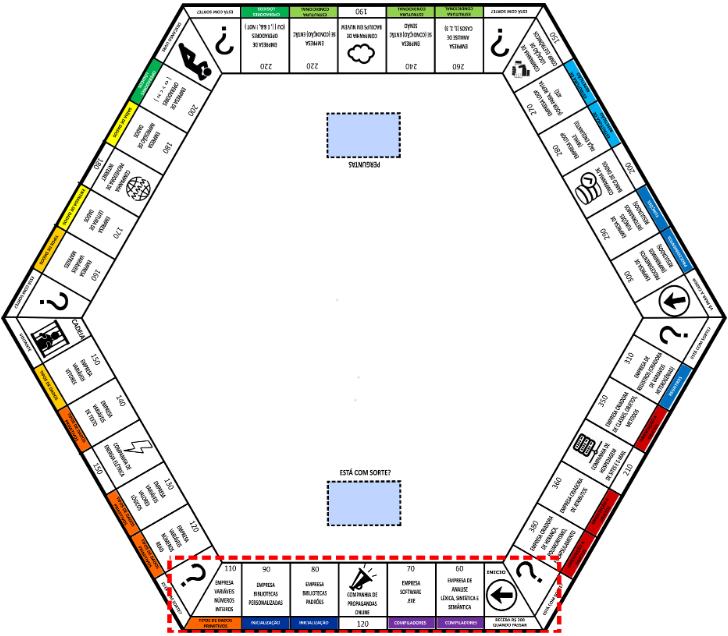
\includegraphics[width=0.8\textwidth]{images/prog-poly.png}
	\legend{Fonte: \cite{nascimento2022prog}}
	\label{fig:prog_poly}
\end{figure}

